% This is "sig-alternate.tex" V2.0 May 2012
% This file should be compiled with V2.5 of "sig-alternate.cls" May 2012
%
% This example file demonstrates the use of the 'sig-alternate.cls'
% V2.5 LaTeX2e document class file. It is for those submitting
% articles to ACM Conference Proceedings WHO DO NOT WISH TO
% STRICTLY ADHERE TO THE SIGS (PUBS-BOARD-ENDORSED) STYLE.
% The 'sig-alternate.cls' file will produce a similar-looking,
% albeit, 'tighter' paper resulting in, invariably, fewer pages.
%
% ----------------------------------------------------------------------------------------------------------------
% This .tex file (and associated .cls V2.5) produces:
%       1) The Permission Statement
%       2) The Conference (location) Info information
%       3) The Copyright Line with ACM data
%       4) NO page numbers
%
% as against the acm_proc_article-sp.cls file which
% DOES NOT produce 1) thru' 3) above.
%
% Using 'sig-alternate.cls' you have control, however, from within
% the source .tex file, over both the CopyrightYear
% (defaulted to 200X) and the ACM Copyright Data
% (defaulted to X-XXXXX-XX-X/XX/XX).
% e.g.
% \CopyrightYear{2007} will cause 2007 to appear in the copyright line.
% \crdata{0-12345-67-8/90/12} will cause 0-12345-67-8/90/12 to appear in the copyright line.
%
% ---------------------------------------------------------------------------------------------------------------
% This .tex source is an example which *does* use
% the .bib file (from which the .bbl file % is produced).
% REMEMBER HOWEVER: After having produced the .bbl file,
% and prior to final submission, you *NEED* to 'insert'
% your .bbl file into your source .tex file so as to provide
% ONE 'self-contained' source file.
%
% ================= IF YOU HAVE QUESTIONS =======================
% Questions regarding the SIGS styles, SIGS policies and
% procedures, Conferences etc. should be sent to
% Adrienne Griscti (griscti@acm.org)
%
% Technical questions _only_ to
% Gerald Murray (murray@hq.acm.org)
% ===============================================================
%
% For tracking purposes - this is V2.0 - May 2012

\documentclass{sig-alternate}
\usepackage{setspace}

\renewcommand{\baselinestretch}{1.5} 
\usepackage{textcomp,upquote,listings, color}
\usepackage{booktabs}
 \definecolor{codegreen}{rgb}{0,0.6,0}
\definecolor{codegray}{rgb}{0.5,0.5,0.5}
\definecolor{codepurple}{rgb}{0.58,0,0.82}
\definecolor{backcolour}{rgb}{0.95,0.95,0.92}
 
\lstdefinestyle{mystyle}{
    backgroundcolor=\color{backcolour},   
    commentstyle=\color{codegreen},
    keywordstyle=\color{magenta},
    numberstyle=\tiny\color{codegray},
    stringstyle=\color{codepurple},
    basicstyle=\footnotesize,
    breakatwhitespace=false,         
    breaklines=true,                 
    captionpos=b,                    
    keepspaces=true,                 
    numbers=left,                    
    numbersep=5pt,                  
    showspaces=false,                
    showstringspaces=false,
    showtabs=false,                  
    tabsize=3
}
 
\lstset{style=mystyle}
\lstset{upquote=true}
\begin{document}
%
% --- Author Metadata here ---
\conferenceinfo{WOODSTOCK}{'97 El Paso, Texas USA}
%\CopyrightYear{2007} % Allows default copyright year (20XX) to be over-ridden - IF NEED BE.
%\crdata{0-12345-67-8/90/01}  % Allows default copyright data (0-89791-88-6/97/05) to be over-ridden - IF NEED BE.
% --- End of Author Metadata ---
\title{ Citations Network Proposal}
\subtitle{The art of information retrieval and visualization}

%
% You need the command \numberofauthors to handle the 'placement
% and alignment' of the authors beneath the title.
%
% For aesthetic reasons, we recommend 'three authors at a time'
% i.e. three 'name/affiliation blocks' be placed beneath the title.
%
% NOTE: You are NOT restricted in how many 'rows' of
% "name/affiliations" may appear. We just ask that you restrict
% the number of 'columns' to three.
%
% Because of the available 'opening page real-estate'
% we ask you to refrain from putting more than six authors
% (two rows with three columns) beneath the article title.
% More than six makes the first-page appear very cluttered indeed.
%
% Use the \alignauthor commands to handle the names
% and affiliations for an 'aesthetic maximum' of six authors.
% Add names, affiliations, addresses for
% the seventh etc. author(s) as the argument for the
% \additionalauthors command.
% These 'additional authors' will be output/set for you
% without further effort on your part as the last section in
% the body of your article BEFORE References or any Appendices.

\numberofauthors{2} %  in this sample file, there are a *total*
% of EIGHT authors. SIX appear on the 'first-page' (for formatting
% reasons) and the remaining two appear in the \additionalauthors section.
%
\author{
% You can go ahead and credit any number of authors here,
% e.g. one 'row of three' or two rows (consisting of one row of three
% and a second row of one, two or three).
%
% The command \alignauthor (no curly braces needed) should
% precede each author name, affiliation/snail-mail address and
% e-mail address. Additionally, tag each line of
% affiliation/address with \affaddr, and tag the
% e-mail address with \email.
%
% 1st. author
\alignauthor
Minh .H Nguyen \\
       \affaddr{International University of Vietnam}\\
       \email{minh.ng0611@gmail.com}
% 2nd. author
\alignauthor
Phat C. Thach \\
       \affaddr{International University of Vietnam}\\
       \email{webmaster@marysville-ohio.com}
  }
% There's nothing stopping you putting the seventh, eighth, etc.
% author on the opening page (as the 'third row') but we ask,
% for aesthetic reasons that you place these 'additional authors'
% in the \additional authors block, viz.

% Just remember to make sure that the TOTAL number of authors
% is the number that will appear on the first page PLUS the
% number that will appear in the \additionalauthors section.
{\setstretch{1.2}

\maketitle
\begin{abstract}
This paper provides a sample of a \LaTeX\ document which conforms,
somewhat loosely, to the formatting guidelines for
ACM SIG Proceedings. It is an {\em alternate} style which produces
a {\em tighter-looking} paper and was designed in response to
concerns expressed, by authors, over page-budgets.
It complements the document \textit{Author's (Alternate) Guide to
Preparing ACM SIG Proceedings Using \LaTeX$2_\epsilon$\ and Bib\TeX}.
This source file has been written with the intention of being
compiled under \LaTeX$2_\epsilon$\ and BibTeX.

The developers have tried to include every imaginable sort
of ``bells and whistles", such as a subtitle, footnotes on
title, subtitle and authors, as well as in the text, and
every optional component (e.g. Acknowledgments, Additional
Authors, Appendices), not to mention examples of
equations, theorems, tables and figures.

To make best use of this sample document, run it through \LaTeX\
and BibTeX, and compare this source code with the printed
output produced by the dvi file. A compiled PDF version
is available on the web page to help you with the
`look and feel'.
\end{abstract}

\terms{

This section describes terms used in this study.

OM : Object-Mapping 

ORM : Object-Relational Mapping 

ODM : Object-Document Mapping 

OGM : Object-Graph Mapping 

CINAS : Citations Network Analysis

RDBMS : Relational Database Management System 

RDB : Relational Database

GDB : Graph Database

USPTO : United States Patent and Trademark Office }

\keywords{Citation Network Analysis, Data Mining, Patent}

\section{Introduction}
A \textbf{patent} is an exclusive right granted for an invention, which is a product or a process that provides, in general, a new way of doing something, or offers a new technical solution to a 
problem [1]. Documentation of a patent provides technological, legal, commercial information about the concerned technical solution to a problem. The information regarding each patent is publicly available online and rapidly accumulated along the time. Not only the USPTO but also does Google make patent and trademark public data available to the public in bulk form so that the data can be used to load into databases or other analytical tools for research and analysis (USPTO, 2012). Hence, exploitation of such information might brings significant benefits to the technology development of a nation - both developing and developed.

The purpose of this study was to proposed the structure, called CINAS, for storing patent information and extract trivial knowledge. In addition, we also measure performances of CINAS's storage, which was implemented based on two different databases, namely MongoDB and Neo4j. The rest of the report is organized as follows: Related works, including similar research on CINAS's implementation using RDBMS are reviewed in section 2. Section 3 gives introduction to CINAS, choices of technology and approach of design are also explained briefly. CINAS's detailed implementations are elaborated in section 4. Preliminary results are presented in section 5. Finally, this work is concluded in section 6

\section{Background and related work}
A summer project held by group of researchers from University of Illinois at Urbana-Champaign provides a database of USPTO patent from 1976 to 2012. According to the authors,  the main goal was to obtain online patent bulk data automatically and parse the data using self-written Python program; then all the processed data are populated into MySQL database. Two main types of patents, namely Patent Grants and Patent Application Publication, are parsed by its corresponding parsers, Grants Parser and Publications Parser respectively. In addition, a Source parser was provided to assist in crawling available links.

The obtained results, however, were only able to show trending in publishing two types of patent, some classification statistics and to some extents, did not give in-depth knowledge. Besides, the main aim of the entire project was solely focused on constructing the database, this lead to to these inevitable facts:

\begin{itemize}
\item Database construction's process was heavily designed to convert and store patent data, the method of transforming stored data into meaningful knowledge has not been mentioned. It's not viable to store data without particular needs, this approach would then be inflexible and requires additional layers of extraction to retrieve desired data for analysis.
\item Source code was lack of detail explanation on reusable module and properly out-of-dated since 2012.
\item Grant Parser was implemented with ElementTree module which would load the entire XML file onto memory. This method is inefficient as it scales linearly with size of dataset and memory's consumption.
\item Since patents are hybrid-structure files, MySQL, being as a relational database, doesn't support for text search and unstructured data within patent such as text descriptions and claims. 
\end{itemize}

There is also an online solution providing fine-tuned patent database which can be downloaded from Institute of Intellectual Property \footnote{https://database.iip.or.jp/patentdb/index\_e.php}. As stated by IIP, data is exhibited only for the purpose of research spread of patent statistics, and cannot be used for any commercial purpose. Besides, relying on third party solution would only increase the conversion time, thus we decided to handle raw XML files from USPTO.

In this study, we propose CINAS as an alternative solution that are flexible and eliminates the disadvantages of the previous studies.

\section{Introduction to CINAS}
CINAS initially aims to provide more flexible and scalable solution for big patent data. Similar to other system, the process of analyzing patents following CINAS are explained as follow:

\begin{itemize}
\item Extracting valuable information
\item Inserting into database
\item Exporting the information
\end{itemize}

It's important to note that CINAS is designed to be DBMS-independent. Specifically, the framework has special connectors working as drivers to different databases and thus, can fully take advantages of crossing-database's characteristics. For example, to analyze a citation network in which contains nested relationship and thousand of nodes,  Neo4j is far superior than RDBMS. Nonetheless, Neo4j is remarkably slow when it comes to big data as it stores addition attributes in the relationships between nodes and presents more complicated relationships between each node in comparison to RDBMS. Another example is to analyze text-based field where MongoDB would take primary place because it has no schema enforced on data. No schema would also mean no joinning cost in term of relational and hence, provide more speed. 

Since CINAS is DBMS-independent, it can work well with wide ranges of DBMS to achieve desirable results. In this study, we will present the method of obtaining citation network using Neo4j as backend. Furthermore, we also show how valuable data can be extracted from MongoDB. Last but not least, due to having restricted functionality, the relational database is out of this study's scope.

The dramatical trade-off of this approach is that it would cost more memories, load-balance to maintain two different DBMS system within one host and hence, reducing overall speed. Having thought of that, we implemented CINAS using RESTful APIs to partially address those issues, we also compare the pros and cons with the ORM approach for references in implementation section. Even though it cannot overcome the speed of using ORM with direct-connection to the storage, it's worth mentioned in term of scalability.
\subsection{Neo4j }
Being a world-leading graph database, Neo4j has all the functionalities we need to accomplish our network. A graph database stores data in a graph, the most generic of data structures, capable of elegantly representing any kind of data in a highly accessible way. The simplest possible graph is a single Node, a record that has named values referred to as Properties. A Node could start with a single Property and grow to a few million Properties, though that can get a little awkward. Apart from properties and relationships, nodes can also be labeled with zero or more labels.

Graph Database differs from RDB in the sense that a node itself is a "thing", not a table that holds many records. This provides a level of flexibility to represent data closer to the real world entity. Considering the following example where GDB overwhelms our traditional RDB, that's in a citation networks a patent is cited by many patents. Traditionally, RDB would maintain only single table, named Patent, with each record has an additional column to store foreign key. However, the fact that many patents can cite a single patent and a patent can be referred by many patents would leave us an M-to-N relationship and require a creation of second table. Suppose citations are limited to 1000 patents, which means cited patents and patents are reachable within our database, and each patent can refer up to 1000 patents. Clearly, 1000000 records should be stored inside our second table. Therefore, representing such a nested relationship with tabular system is not a scalable practice since we have more than millions of patents. The above problem can be addressed with 1000 nodes and 2000 relationship in GDB, this is much similar to what we usually think.

An additional important feature in GDB is relationship's weight, this offers more accurate ways to determine the relationship between each entity. 

\subsection{MongoDB}
MongoDB  is an open-source document database, and the leading NoSQL database. MongoDB deploys BSON as an primary data representation and therefore improve speed of traverse through JSON file. BSON, short for Binary JSON, is the binary-encoded version of JSON-like documents. In other words, it adds extensions for data types such as integer or date that are not part of JSON specification. JSON is a self-describing, human readable data format. Originally designed for lightweight exchanges between browser and server, it has become widely accepted for many types of applications. JSON documents are particularly useful for data management for several reasons. A JSON document is composed of a set of fields which are themselves key-value pairs. This means each JSON document carries its own human readable schema design with it wherever it goes, allowing the documents to easily move between database and client applications without losing their meaning. Detailed explanations for JSON and BSON will not be discussed in this study.

A record in MongoDB is a document, which is a data structure composed of field and value pairs. MongoDB documents are similar to JSON objects. The values of fields may include other documents, arrays, and arrays of documents. The advantages of using documents are:
\begin{itemize}
\item Documents (i.e. objects) can be defined with native data types that can be seen in many programming languages. E.x: Date, String, Integer
\item Embedded documents and arrays reduce need for expensive joins.
\item Dynamic schema supports fluent polymorphism.
\end{itemize}

\subsubsection{Downfall of Normalization }
The immediate and fundamental difference between MongoDB and an RDBMS is the underlying data model. A relational database structures data into tables and rows, while MongoDB structures data into collections of JSON documents. The ability to support arrays is an especially helpful feature; it simplifies the way my application interfaces with the database and helps me avoid a complicated database schema. Consider the complexity of supporting a repeating group in a properly normalized table structure. To represent the same data object in a single table row would like like this:
\begin{table}[htb]
\begin{tabular}{|c|c|l|} \hline
PatentID&Title&Classification\\ \hline
1& "Snack"& "D1, D2, D3"\\ \hline
\end{tabular}
\centering
\caption{Patent Table}
\end{table}
Aggregation and updating specific classification for a comma separated list might pose serious problems and extra works. The first normalization was designed to avoid such problems by dividing each class into different records.

\begin{table}[htb]
\begin{tabular}{|c|c|l|} \hline
PatentID&Title&Classification\\ \hline
1& "Snack"& "D1"\\ \hline
1& "Snack"& "D2"\\ \hline
1& "Snack"& "D3"\\ \hline
\end{tabular}
\centering
\caption{1st Normalized Patent Table}
\end{table}

We create a data redundancies that make us susceptible to anomalies. An example is to issue update command using SQL query :

\begin{lstlisting}[caption=Json Example]
UPDATE Patent 

SET Title = "New Snack"  

WHERE PatentID = 1 

AND Classification = "D1"
\end{lstlisting}

\begin{table}[htb]
\begin{tabular}{|c|c|l|} \hline
PatentID&Title&Classification\\ \hline
1& "New Snack"& "D1"\\ \hline
1& "Snack"& "D2"\\ \hline
1& "Snack"& "D3"\\ \hline
\end{tabular}
\centering
\caption{1st Normalized Patent Table}
\end{table}

This happens because the table fail to qualify a 2nd Normalization Form. Classification is not functionally dependent on Title since there are three titles with different classes. Hence, we need to normalize data into 2 separated tables.

\begin{table}[htb]
\centering
\begin{tabular}{|c|c|l|} \hline
PatentID&Title\\ \hline
1& "Snack"\\ \hline
\end{tabular}

\begin{tabular}{|c|c|l|} \hline
PatentID&Classification\\ \hline
1& "D1"\\ \hline
1& "D2"\\ \hline
1& "D3"\\ \hline
\end{tabular}
\centering

\centering
\caption{2nd Normalized Patent Tables}
\end{table}

This structure prevents the anomaly, but introduces a new set of problems. The new schema has become much more complex, and we have lost any semantic understanding of stored objects. By adhering to these two normal forms, we've also entered the realm of cross-table joins and the need to enforce ACID transactions across multiple tables. The enforcement of referential integrity in multi-row, multi-table operations will require concurrency controls, increasing overhead and affecting performance.

MongoDB avoids these complications through the use of a document data model. The JSON document forms a more natural representation on the data than the normalized schema. It achieved this by allowing the embedding of related data via arrays and sub-documents within a single document - thus eliminating the need for JOINs, referential integrity and multi-record ACID transactions.

\begin{lstlisting}[caption=Json Example]
{
	{
	"_id" : ObjectId("528ba7691738025d11aab772"),
	"patid" : 1,
	"title": "Snack",
	"classification" : ["D1", "D2", "D3"]
	}
}
\end{lstlisting}

\subsection{OM and REST services}

Object Mapping is an layer over database to assist querying and managing data using an object paradigm. The pros of this method is that it hides the database query language syntax away from logic code. Following this manner, data models are gathered in one place and it's easier to update, maintain and reuse the code. Every databases have its different mapping methodology. For example, relational database will need object-relational- mapping while object-document mapping serves as driver between web applications with document-oriented database. The drawback of using OM is that OM tools generally stem from the high level of abstraction obscuring what is actually happening in the implementation code. Also, heavy reliance on OM software has been reported as a major factor in producing poorly designed databases. Furthermore, as we stated CINAS is database-indenpent, it's better to exchange data over more popular format such as JSON instead of binding to a specific database's language. Last but not least, OM does not provide neither enhanced security sevices as it has its own connection to the database, nor load-balancing. This would leave more works on the database's side.

REST, for REpresentational State Transfer, is a simple stateless architecture generally running over HTTP. REST has become the norm in past decades\footnote{http://searchsoa.techtarget.com/feature/Gartner-analyst-REST-APIs-gain-added-importance-in-application-integration-design
} as the majority of developers would prefer this scalable solution. Considering the fig below,
\begin{figure}[htb]
\centering
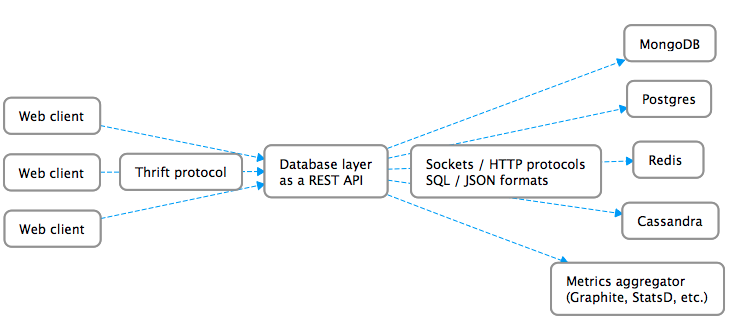
\includegraphics[width=80mm,scale=10]{restapi.png}
\caption{ RestAPI }
\end{figure}

the boons of REST services are:
\begin{itemize}
\item It's simpler in comparison to OM as it only uses GET, PUT, POST, DELETE and PATCH to communicate with the web services.
\item  Switching some data from Postgres to MongoDB or sharding in MongoDB, etc. could be hidden as internals of this layer. This copes well with our requirement for database-independence.
\item Providing middle layer would also enhance rate-limiting, monitoring and scalability - and Database's memory leaks, etc. would not affect other parts of the system.
\end{itemize}

Despite having favors for REST, the services are generally suffer from performance as it wraps data through an additional layer and also provide an abstraction over databases.
\subsection{Gephi}
Unfortunately, Neo4J visual browser only supports up to 1000 rows\footnote{http://stackoverflow.com/questions/26031795/resultset-too-large-over-1000-rows-in-neo4j-browser} and the performance becomes inconsistent as data grows, we chose Gephi to alternatively visual our network. Gephi is a collaborative open-source project. It has been built to be easily extended and reused. Like Photoshop but for data, the user interacts with the representation, manipulate the structures, shapes and colors to reveal hidden properties. The goal is to help data analysts to make hypothesis, intuitively discover patterns, isolate structure singularities or faults during data sourcing \footnote{http://gephi.github.io/features/}. We will be using Gephi to perform analysis on our citations network.

\subsection{R-Studio}

R-Studio is an integrated development  environment for R\footnote{http://www.rstudio.com/products/rstudio/features/}. Its features includes effective data handling and graphical facilities for data analysis, as well as functionality for wide variety of statistical (linear and nonlinear modelling, classical statistical tests, time-series analysis, classification ) \footnote{http://www.r-project.org/} . Therefore, R is chosen to demonstrate what knowledge we can learn from data statistic, which will be extracted from MongoDB.

\section{CINAS's Implementation }

Either using Neo4J or MongoDB alone would be adequate to achieve the same results. However, in this study, we will develop CINAS using wide ranges of databases and approaches to effectively measure the differences.
\subsection{Conceptual Model}
We want to build a system that can store and analyse patents from USPTO. A patent contains an unique Publication number, Publication type, Application number, Publication date, Filling date, Priority date, Fee status (Paid or Free), Title, Length of grant (years), Classification and some of its contents include Abstract, Images, Description and Claims. A patent may or may not cite any other patents; and it may or may not be cited by other patents. A patent must be invented by at least one Inventor, be applied by only one Applicant, be assigned for at least one Assignee and be examined by at least one Examiner. The system will identify Inventor, Applicant, Assignee and Examiner by four attributes, which are their first name, last name, city and country.

\begin{figure}[htb]
\centering
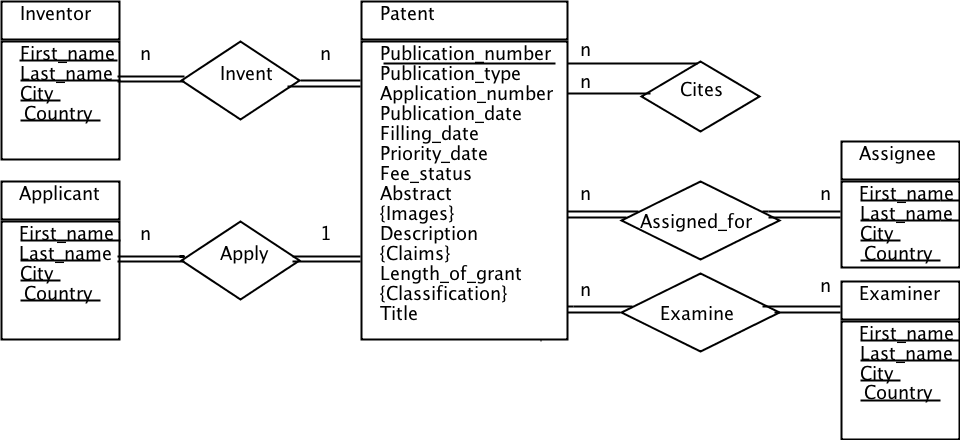
\includegraphics[width=80mm,scale=10]{erd.png}
\caption{ PatenDB Conceptual Model}
\end{figure}

Due to limited resources, instead of implementing the complete system, we chose the simple modelling to convey the operations of CINAS. The database is called PatentDB which has only two entities, inventor and patent. The relationship between entities and its attribute are illustrated in fig.1. 

\begin{figure}[htb]
\centering
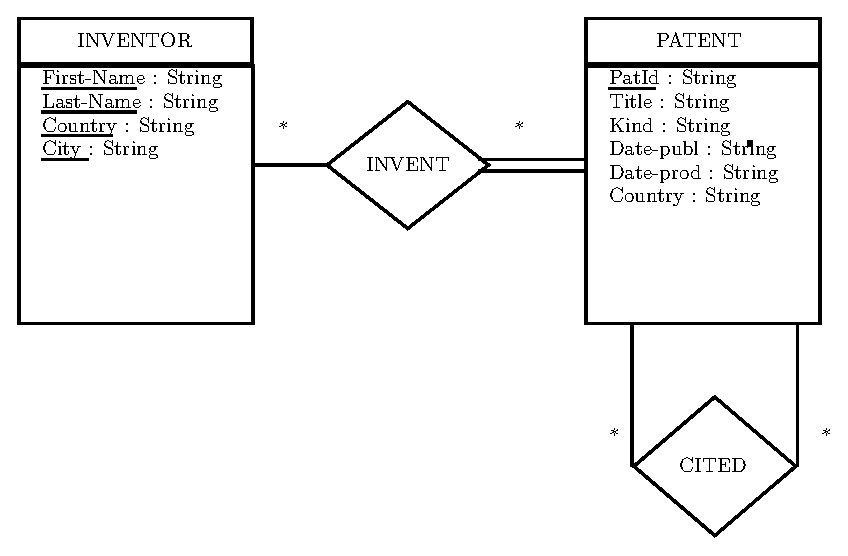
\includegraphics[width=80mm,scale=10]{conceptual_model.eps}
\caption{ Demo Conceptual Model}
\end{figure}

Rules are simple as follow:

\begin{itemize}
  \item An inventor may invent many patents and many inventors can work on the same one
  \item A patent might be cited by other patents or may refer to many patents
\end{itemize}

The problem arises when we present the relationship between citations and patents and whether we should treat them differently. In fact, citations are references to the other patents, we can think of them as foreign keys in relational way. Therefore, it's more plausible to treat them as one entity, called Patent. Another issue we can not overlook is the creation of citations and patents, which should be create first ? The answer is obviously to create citations as patents with dummy information so that we can make a reference first, and then we overwrite the content once we process the corresponding patent later. Following this manner, we can obtain a more comprehensive result. Insight of implementation are described in section 4.3.2.

\subsection{Logical Model}
\subsubsection{Mapping to Graph Logical Model}

\begin{figure}[htb]
\centering
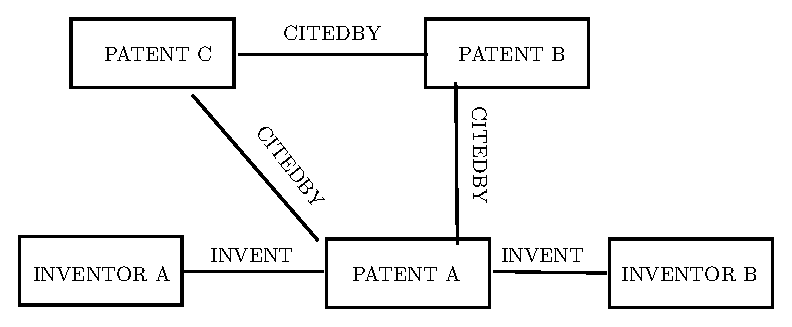
\includegraphics[width=80mm,scale=10]{neo4jgraph.eps}
\caption{ PatenDB Conceptual Model}
\end{figure}

\subsubsection{Mapping to Document-oriented Logical Model}
With MongoDB, you may embed related data in a single structure or document. These schema are generally known as "denormalized" models, and take advantage of MongoDB's rich documents. Consider the following diagram:
\begin{lstlisting}[caption=Document-oriented schema]
patent_schema = {
    kind : string, 
    date-published : string, 
    number-of-claims : integer, 
    country : string, 
    patid : string,
    main-classification : string,
    title : string,
    app-number : string, 
    citations : [ { patid : string }, { patid : string }]
    date-produced : string, 
    inventors:[
        { city : string,  last-name : string, country : string, first-name : string },
	{ city: string,  last-name : string, country : string, first-name : string }
     ]       
}

inventor_schema={
    city : string, 
    last-name : string, 
    country : string, 
    first-name : string
}
\end{lstlisting}

In general, embedding provides better performance for read operations, as well as the ability to request and retrieve related data in a single database operation. Embedded data models make it possible to update related data in a single atomic write operation. We use embedded schema of inventor inside patent's schema.

However, embedding related data in documents may lead to situations where documents grow after creation. Document growth can impact write performance and lead to data fragmentation. We would use reference for patent's citations. However, client-side applications must issue follow-up queries to resolve the references. In other words, normalized data models can require more round trips to the server.


\subsection{CINAS Structure}
In this section, we will describe each component of CINAS in detail and also discuss design methodology. Fully written in Python, CINAS consists of 2 main modules:
\begin{enumerate}
 \item Firstly, XML Parser Module to parse the input XML file into JSON format
 \item DB Client would then load of JSON format files to populate it into Database.
\end{enumerate}
REST services are provided by external resources.
\begin{figure}[htb]
\centering
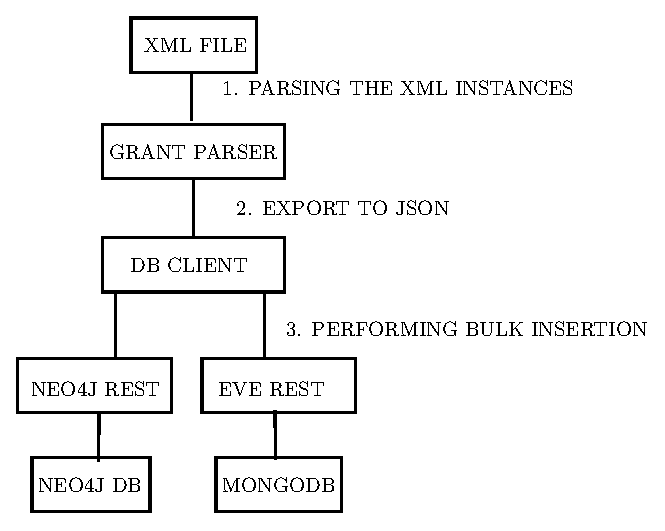
\includegraphics[width=80mm,scale=0.1]{cinasstruct.eps}
\caption{ CINAS ARCHITECTURE}
\end{figure}
\subsubsection{XML Parser Module}
There are two approaches in designing XML parsers. Either one may choose DOM method, which load the entire file onto memory using ElementTree, or line by line processing by SAX. Even though the former method is remarkably simpler and faster, it is susceptible to memory consumption. As data grows big, implementing parser using DOM method is not plausible. Fortunately, the latter is well suit for parsing big data by design and thus, will be implemented in CINAS.

\begin{figure}[htb]
\centering
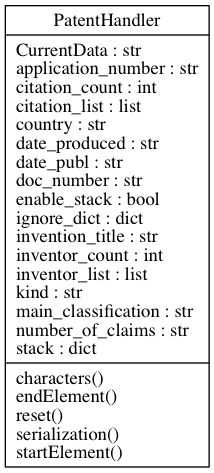
\includegraphics[width=40mm,scale=10]{handler.png}
\caption{ Patent Handler Class Diagram}
\end{figure}

The core of Grant Parse script is PatentHandler class, class diagram of it is shown in figure 5. It mainly used to hold data that parsed from each XML instance. Since SAX Parser only read XML line by line, it's reasonable to keep track of processing tag using stack. All of the function prototypes and attributes are carefully documented in Appendix A. In brief, Grant Parser currently works following this procedure
\begin{enumerate}
 \item Load XML file and break it down into separated XML instances
 \item Parse each XML instance into patent handler. For each tag with nested tags, enable stack to store adjacent data.
 \item Tags that are explicitly defines in ignore list will be left out during parsing. Upon completion, reset the patent handler for new instance
 \item Finally, an option to export the entire file to JSON format is available if chosen.
\end{enumerate}

An implementation using DOM tree is also documented solely for benchmark's comparison and thus, detailed explanations are beyond the scope of this study.

\subsubsection{DB Client Module}
Instead of using OM for particular database, we chose to deploy REST services as mean of communication with our backends. It's complicated to wrap OM around another OM, but it's simple to wrap data around HTTP response and request before forwarding. Therefore this approach provides more scalable solution than OM. Despite the fact that this approach might limit the performance speed, it's worth a trade-off for being more extendable. The figure 6 illustrate class diagram of our DB Client module.

\begin{figure}[htb]
\centering
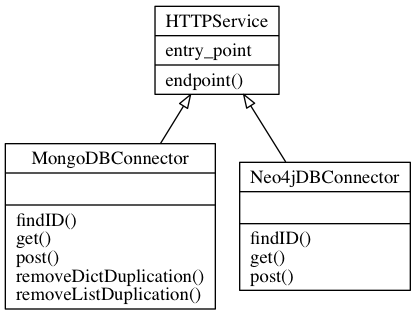
\includegraphics[width=80mm,scale=10]{db_client.png}
\caption{ DB Client Class Diagram}
\end{figure}

The idea is to create an abstract layer to hide the presence of multi-databases systems. Instead of choosing ODM for MongoDB or OGM for Neo4J, we created an data layers to a enhance the transparency. For example, to issue a POST request to whatever the backend is, developers currently only need to concern the differences between resources and query format ( commonly json ). The complexity underlying will be handled by each corresponding connectors. As can be seen from figure 6, all the fundamental HTTP methods are implemented in HTTPServices. MongoDBConnector and Neo4JDBConnector inherit private methods from its parent, insight of private functions are documented in Appendix A. 

It's important to note that we need to handle with cares for MongoDB as it's susceptible to data redundancy and inconsistency due to being no schema DB. In addition, MongoDB requires an object ID to make a legitimate references. In specific, for a patent to make references, it should store the objectID of patent instead of proposed patent ID. From our opinions, we think this is unnecessary and generate extra workload for conversions. Hence, we use embedded to represent the relationships between patent. 

Regarding the duplication in MongoDB, considering this case where patent 08852195 actually refer to WO2005/069809 twice at line 329 and line 330\footnote{http://www.directorypatent.com/US/08852195.html}, it's inevitable that we might have data redundancies to some extents. Even though it's more acceptable to treat them as one entity, we would consider it in our next stage of implementation due to time constraint.

The procedure of POST in MongoDB is:
\begin{enumerate}
 \item Load all data from JSON file
 \item Construct list of citations from group of patent
 \item Validate uniqueness within the list. When we insert using bulk insertion, 3 patents might references the same patent and this will culminate in data duplication in DB. We can not overlook this problem.
 \item Appending statements into query. Then, perform 1st POST these citations 
 \item If the uniqueness is violated, the response code from EVE server will determine the next step. If error response with duplicates found, we remove it from the list and resend it again.
 \item Finally, we perform an overwrite PUT for any individual patent. This step must be linearly execute to guarantee that all the dummy patents, which are created using citations, will be updated with information.
\end{enumerate}

The procedure of POST in Neo4J is much more simpler, since Neo4J has an overwrite operation called "MERGE" and allow developers to execute it through cypher endpoint. Therefore, it reduces the need for extra validation:
\begin{enumerate}
 \item Load all data from JSON file
 \item Construct list of citations from group of patent
 \item Appending statements into query. Then, perform POST these citations 
 \item Finally, we perform another POST for list of patents.
\end{enumerate}

\subsubsection{External Modules}
CINAS also has some utilities provided out-of-box to improve the readability and statistical measurements. 
\begin{enumerate}
 \item \textbf{benchmark.py} is a small library that supplies apis for benchmark measurements
 \item \textbf{generate\_csv.py} retrieves data from Neo4J and generate two csv files of nodes and links for citations network. In specific, \textbf{nodes\_network.csv} contain nodes, which might be inventors or patents, and the link between them is stored in \textbf{links\_network.csv}. These csv will then be manually loaded into Gephi to analyze the results. Figure 7 is work flow of analyzing data from Neo4J. All  APIs and variables are well documented in Appendix A.
 
\end{enumerate}
\begin{figure}[htb]
\centering
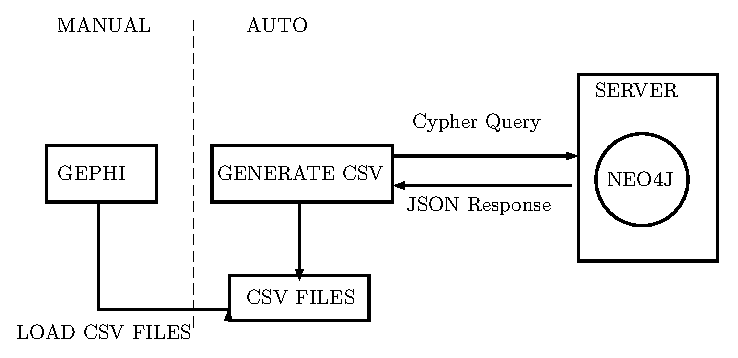
\includegraphics[width=90mm]{generate.eps}
\caption{ CSV Generator Class Diagram}
\end{figure}
\begin{table*}
\begin{tabular}{|c|c|l|} \hline
 Class & Descriptions \\ \hline
D99 & MISCELLANEOUS \\ \hline
D34 & MATERIAL OR ARTICLE HANDLING EQUIPMENT\\ \hline
D32 & WASHING, CLEANING, OR DRYING MACHINE\\ \hline
D30 & ANIMAL HUSBANDRY\\ \hline
D29 & EQUIPMENT FOR SAFETY, PROTECTION, AND RESCUE (1)\\ \hline
D28 & COSMETIC PRODUCTS AND TOILET ARTICLES\\ \hline
D26 & LIGHTING\\ \hline
D25 & BUILDING UNITS AND CONSTRUCTION ELEMENTS\\ \hline
D24 & MEDICAL AND LABORATORY EQUIPMENT\\ \hline
D23 & ENVIRONMENTAL HEATING AND COOLING; FLUID HANDLING AND SANITARY EQUIPMENT\\ \hline
D21 & GAMES, TOYS, AND SPORTS EQUIPMENT\\ \hline
D20 & SALES AND ADVERTISING EQUIPMENT\\ \hline
D19 & OFFICE SUPPLIES, ARTISTS AND TEACHERS MATERIALS\\ \hline
D17 & MUSICAL INSTRUMENTS\\ \hline
D16 & PHOTOGRAPHY AND OPTICAL EQUIPMENT\\ \hline
D15 & MACHINES NOT ELSEWHERE SPECIFIED\\ \hline
D14 & RECORDING, COMMUNICATION, OR INFORMATION RETRIEVAL EQUIPMENT\\ \hline
D13 & EQUIPMENT FOR PRODUCTION, DISTRIBUTION, OR TRANSFORMATION OF ENERGY\\ \hline
D12 & TRANSPORTATION\\ \hline
D11 & JEWELRY, SYMBOLIC INSIGNIA, AND ORNAMENTS\\ \hline
D10 & MEASURING, TESTING OR SIGNALING INSTRUMENTS\\ \hline
D9 & PACKAGES AND CONTAINERS FOR GOODS\\ \hline
D8& TOOLS AND HARDWARE \\ \hline
D7& EQUIPMENT FOR PREPARING OR SERVING FOOD OR DRINK NOT ELSEWHERE SPECIFIED \\ \hline
D6 & FURNISHINGS\\ \hline
D5 & TEXTILE OR PAPER YARD GOODS; SHEET MATERIAL\\ \hline
D4 & BRUSHWARE\\ \hline
D3 & TRAVEL GOODS AND PERSONAL BELONGINGS\\ \hline
D2 & APPAREL AND HABERDASERY\\ \hline
D1 & EDIBLE PRODUCTS\\ \hline
\end{tabular}
\centering
\caption{USPTO - Classification Table}
\end{table*} 
 
\section{Preliminary Results}
Contemporary, CINAS has processed up to 110343 so-called patents. Table 6 show the summarized statistic of patent database.
\begin{table}[htd]
\begin{tabular}{|c|c|l|} \hline
 &Number of Documents\\ \hline
 Duplicated Citations&347 \\ \hline
Patents&3000 \\ \hline
Citations&106996 \\ \hline
Total & 110343\\ \hline
\end{tabular}
\caption{Summarize Table}
\end{table}
From figure 8, it's immediately striking that inventions for MISCELLANEOUS (D99) industry were blossomed in October 2014. In specific, nearly 2500 granted patents ( accounted for nearly 83\%) makes non-trivial goods production industry become the most popular topic among the invention community. In addition, this might signal a competitive field for any inventors that shall want to take part in. On the opposite, classification that are larger than 20 were recorded at lowest level, except for the case of  MEDICAL AND LABORATORY EQUIPMENT (D24), ENVIRONMENTAL HEATING AND COOLING; FLUID HANDLING AND SANITARY EQUIPMENT (D23)
?and LIGHTING(26) where number of inventions are relatively close to those in range of 1x (approx. 100) . In general, involving in these fields might be less competitive than the others. Even though coming in second place of the ladder,RECORDING, COMMUNICATION, OR INFORMATION RETRIEVAL EQUIPMENT's inventions (D14) are accounted for merely 6.66\%, in other words, 15 times smaller than the dominant D99. Interestingly, this also indicates the need for more robust information retrieval system is significant and thus, was main motivation for this study. Following D14 closely was TOOLS AND HARDWARE (D8) which received 150 attentions. Finally, we  also witness the insignificant presence of inventions in various class among 1x and 0x. As promised, statistics and bar chart was computed and generated using R. 
\begin{figure}[htb]
\centering
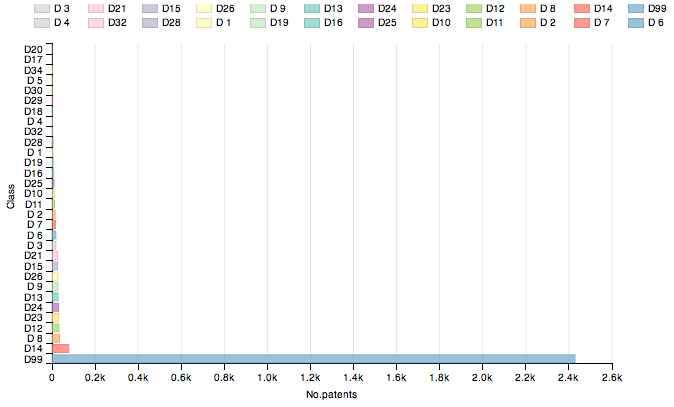
\includegraphics[width=90mm]{rplot-classification.png}
\caption{ Patent Classification October 2014 }
\end{figure}

\subsection{Citations Network}

We also demonstrate citations network on 500 patents instead of 3000 patents due to memory constrain on personal computer. A full view of network consists of inventors, patents, citations and their links are shown in figure 9. 
\begin{figure}[htb]
\centering
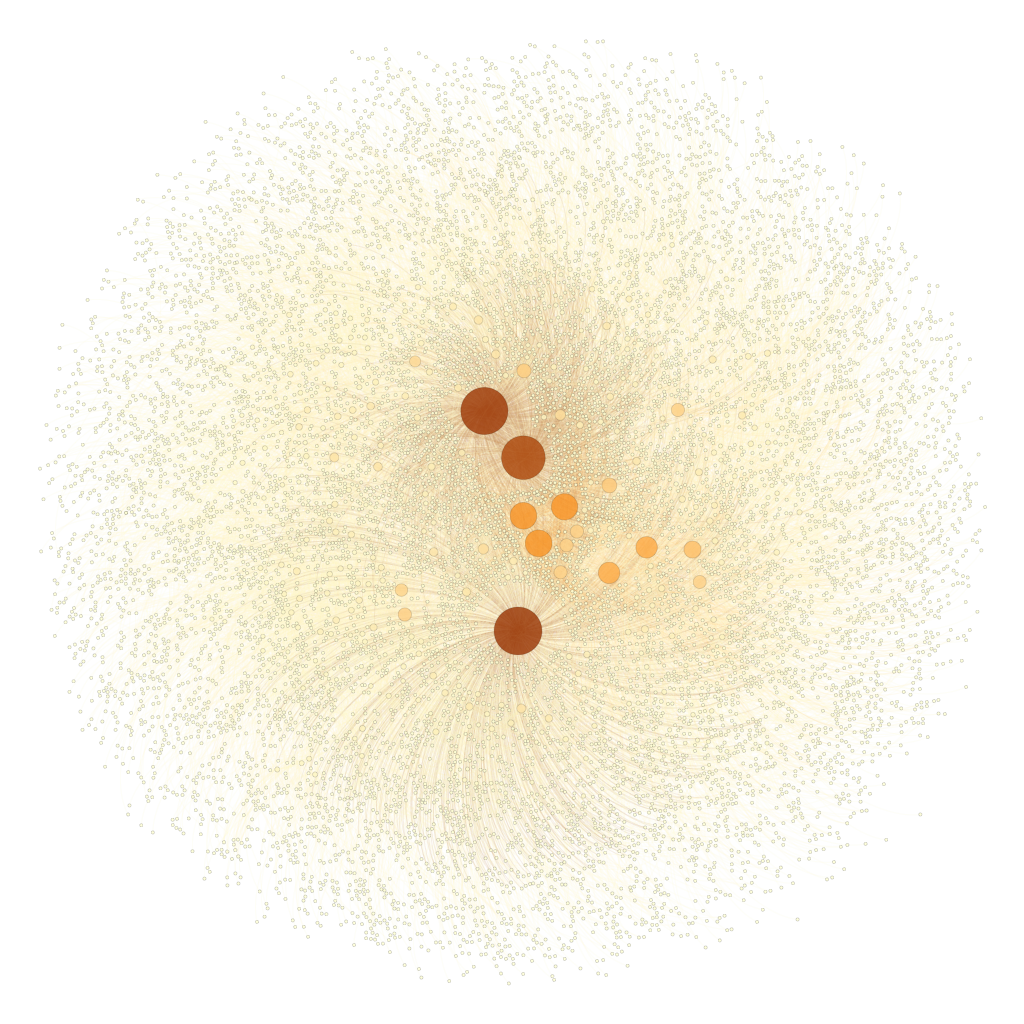
\includegraphics[width=90mm]{citation.png}
\caption{ Patents and Citations October 2014 }
\end{figure}

In this figure, using Gephi as visualization tool to enhance the spatialization within the network, we applied the force-directed layout Fruchterman Reingold to scatter out the node \footnote{http://en.wikipedia.org/wiki/Force\-directed\_graph\_drawing} and Force Atlas to distribute nodes without overlapping \footnote{http://webatlas.fr/tempshare/ForceAtlas2\_Paper.pdf}. Specifically, Bigger nodes will be gather at the central of the graph while nodes with least connections are pushed to the rear area. A closer look at citations network can be observed from figure 10. In particular, we applied ranking by connected component to distinguish group of nodes which have largest number of connections.

\begin{figure}[htp]
\centering
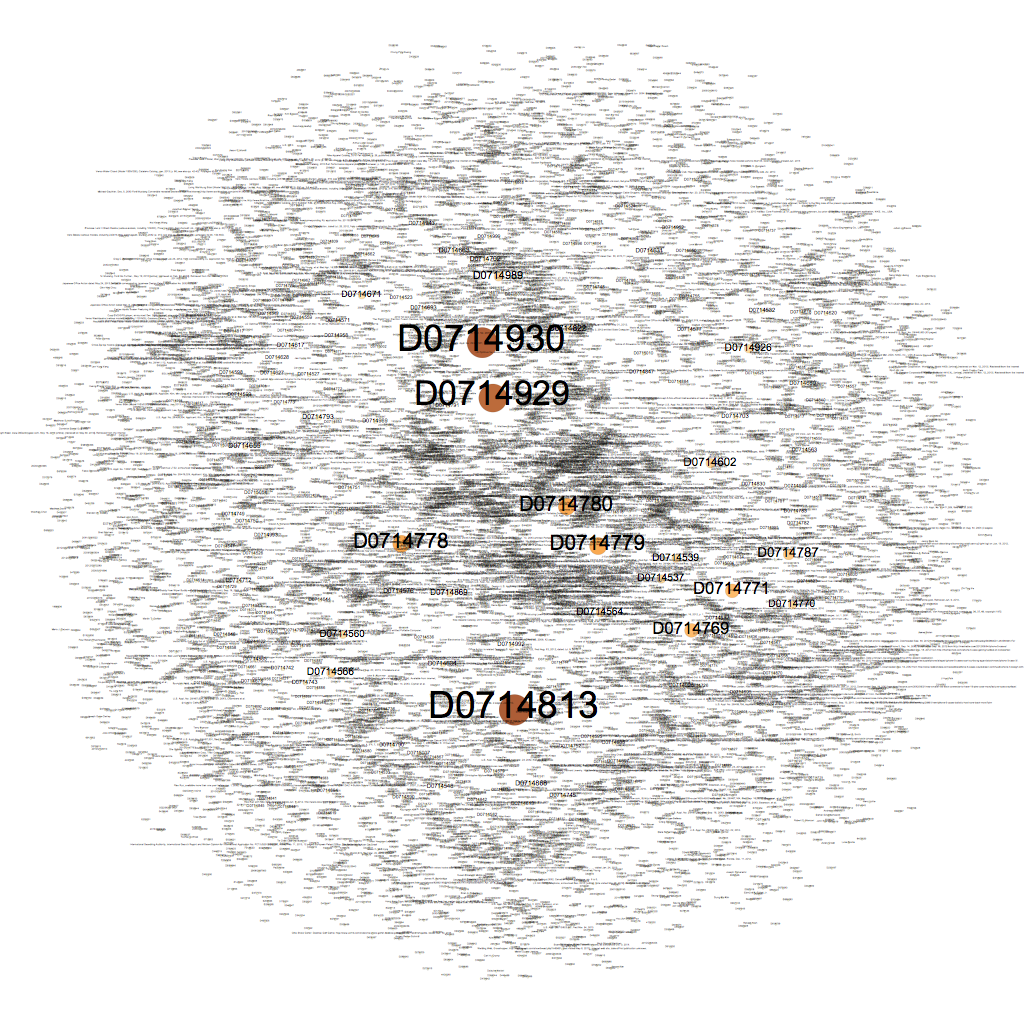
\includegraphics[width=80mm]{citation-label.png}
\caption{ Citations Network October 2014 }
\end{figure}
Ranking by connected components gives us the importances of particular node since not only many inventors connect to it, but also do many inventions actual refer to it as a fundamental foundation.  
\begin{table}[]
\begin{tabular}{|c|c|c|c|}  \hline
 ID&Title&No.citations&Class\\ \hline
 D0714930&Reservoir.for.water.flosser&495&D24\\ \hline
D0714929&Base.for.water.flosser&457 &D24\\ \hline
D0714813&Electronic.camera&517&D14 \\ \hline
\end{tabular}
\caption{Most connected components patents information}
\end{table}
Table 7 shows the information regarding group of most-connected nodes from the graph. Unfortunately, All of them are recently published and thus, we can not observe the case where patent from the past was referred by many patents from this figure.
In figure 11, the edges of the network reflect patents or inventors that are connected to only one node of the graph. Following the connected-components ranking algorithm, we might deduce that they are lack of popularity and feasible knowledge.
 \begin{figure}[!htb]
\centering
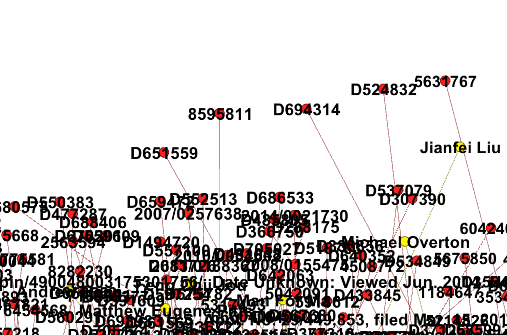
\includegraphics[width=80mm]{endcitation.png}
\caption{ Citations Network Edge October 2014 }
\end{figure}



 \subsection{Inventors Maps}
To measure the activity of inventors community, we classify them based on their regions in figure 12. It's not surprising to witness the outstanding in the field of North America since it's their nation to begin with. However, it's interesting to see that US patents industry also attracts the numerous inventors from different parts of the world, including Asian and Australian. Besides, Russia, despite being second polar of the world in term of economy and currently has oil dispute with American, has no inventors take part in. Overall, the figure might indicate the inventing opportunities in US patent industry from the perspective of the outsiders.
 \begin{figure}[!htb]
\centering
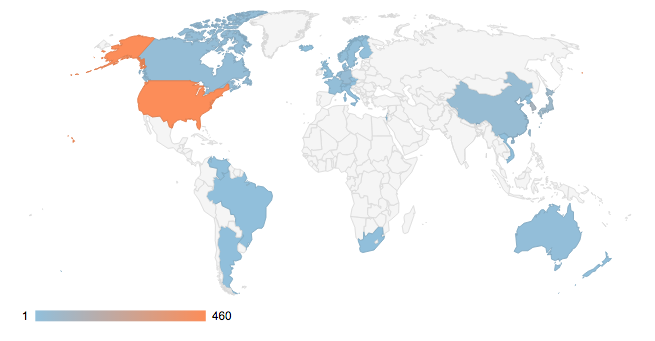
\includegraphics[width=90mm]{inventor-map.png}
\caption{ Geographic of inventors October 2014 }
\end{figure}

 \subsection{Benchmark Neo4J and MongoDB}
 \begin{table}[!ht]
 \centering

\begin{tabular}{lllllll}
\toprule 
    Patents & \multicolumn{1}{c}{Parsing} &\multicolumn{2}{c}{Duplication}\\

    & 
    & Neo4J & MongoDB\\
    \midrule
    $50 + 1224$     & 0.96s   &248.44 & 15.64 \\
    $100 + 2306$  & 1.47s &448.65 & 30.88\\
    $200 + 4439$  & 2.68s &974.57 & 87.55\\
    $300 + 7834$  & 4.42s&1476.65 & 159.04\\
    $400 + 9313$  & 6.48s &2942.61 & 213.21\\
    $500 + 12016$  & 6.99s&2780.16 & 287.58\\
    \bottomrule
\end{tabular}
\caption{Write performance of CINAS}
\end{table}

\section{Conclusions}
This paragraph will end the body of this sample document.
Remember that you might still have Acknowledgments or
Appendices; brief samples of these
follow.  There is still the Bibliography to deal with; and
we will make a disclaimer about that here: with the exception
of the reference to the \LaTeX\ book, the citations in
this paper are to articles which have nothing to
do with the present subject and are used as
examples only.
%\end{document}  % This is where a 'short' article might terminate

%ACKNOWLEDGMENTS are optional
\section{Acknowledgments}
This section is optional; it is a location for you
to acknowledge grants, funding, editing assistance and
what have you.  In the present case, for example, the
authors would like to thank Gerald Murray of ACM for
his help in codifying this \textit{Author's Guide}
and the \textbf{.cls} and \textbf{.tex} files that it describes.

%
% The following two commands are all you need in the
% initial runs of your .tex file to
% produce the bibliography for the citations in your paper.
\bibliographystyle{abbrv}
\bibliography{sigproc}  % sigproc.bib is the name of the Bibliography in this case
% You must have a proper ".bib" file
%  and remember to run:
% latex bibtex latex latex
% to resolve all references
%
% ACM needs 'a single self-contained file'!
%
%APPENDICES are optional
%\balancecolumns
\appendix
%Appendix A
\section{Headings in Appendices}
The rules about hierarchical headings discussed above for
the body of the article are different in the appendices.
In the \textbf{appendix} environment, the command
\textbf{section} is used to
indicate the start of each Appendix, with alphabetic order
designation (i.e. the first is A, the second B, etc.) and
a title (if you include one).  So, if you need
hierarchical structure
\textit{within} an Appendix, start with \textbf{subsection} as the
highest level. Here is an outline of the body of this
document in Appendix-appropriate form:
\subsection{Introduction}
\subsection{The Body of the Paper}
\subsubsection{Type Changes and  Special Characters}
\subsubsection{Math Equations}
\paragraph{Inline (In-text) Equations}
\paragraph{Display Equations}
\subsubsection{Citations}
\subsubsection{Tables}
\subsubsection{Figures}
\subsubsection{Theorem-like Constructs}
\subsubsection*{A Caveat for the \TeX\ Expert}
\subsection{Conclusions}
\subsection{Acknowledgments}
\subsection{Additional Authors}
This section is inserted by \LaTeX; you do not insert it.
You just add the names and information in the
\texttt{{\char'134}additionalauthors} command at the start
of the document.
\subsection{References}
Generated by bibtex from your ~.bib file.  Run latex,
then bibtex, then latex twice (to resolve references)
to create the ~.bbl file.  Insert that ~.bbl file into
the .tex source file and comment out
the command \texttt{{\char'134}thebibliography}.
% This next section command marks the start of
% Appendix B, and does not continue the present hierarchy
\section{More Help for the Hardy}
The sig-alternate.cls file itself is chock-full of succinct
and helpful comments.  If you consider yourself a moderately
experienced to expert user of \LaTeX, you may find reading
it useful but please remember not to change it.
%\balancecolumns % GM June 2007
% That's all folks!
}
\end{document}
